\chapter{Controllo LQR (Linear Quadratic Regulator)}
\label{chap:disturbi_vento}
\label{cap:lqr}
 \label{sec:cap12_1}
 \label{sec:Capitolo 12Wind}

\section{Sintesi del regolatore }
A differenza del classico approccio Proporzionale-Integrale-Derivativo (PID) — il quale opera tipicamente in retroazione sull'uscita (\textit{Output Feedback}), misurando l'errore tra il riferimento e la variabile effettivamente controllata — la logica LQR si basa sulla retroazione completa di stato (\textit{Full State Feedback}). Questo significa che il controllore non si limita a osservare una singola uscita $y(t)$, ma sfrutta l'informazione simultanea di tutte le variabili dinamiche del sistema $\delta\mathbf{x}(t)$ per calcolare l'azione di controllo ottima. Tale approccio multivariabile risulta particolarmente indicato per le dinamiche di volo, in quanto permette di gestire matematicamente e in modo naturale gli accoppiamenti tra i vari stati (come la forte interazione tra velocità, angolo d'attacco e beccheggio). Un passaggio cruciale nella progettazione pratica del sistema consiste nel separare gli ingressi fisicamente comandabili dai disturbi esterni. La dinamica longitudinale completa del velivolo è infatti descritta dall'equazione:
\begin{equation}
    \delta\dot{\mathbf{x}} = A_{long} \delta\mathbf{x} + B_{ctrl} \delta\mathbf{u} + B_{wind} \delta\mathbf{d}
\end{equation}
dove $B_{ctrl}$ rappresenta la matrice di ingresso associata esclusivamente ai veri attuatori fisici a disposizione del sistema (es. manetta ed equilibratore), mentre $B_{wind}$ mappa l'effetto dei disturbi atmosferici, come le raffiche di vento $\delta\mathbf{d}$. Poiché l'algoritmo di controllo non ha autorità sull'atmosfera circostante, la sintesi dell'ottimizzatore LQR deve essere effettuata considerando \textbf{esclusivamente} la sottomatrice $B_{ctrl}$. L'inclusione del termine del vento nel calcolo ottico porterebbe infatti alla genesi di un controllore illogico, che tenterebbe di usare il disturbo come se fosse una superficie di governo.

La legge di controllo retroazionata assume pertanto la forma:
\begin{equation}
    \delta\mathbf{u}(t) = -K \delta\mathbf{x}(t)
\end{equation}
dove $K$ rappresenta la matrice dei guadagni ottimi riferita unicamente agli attuatori fisici.

\subsection{Orizzonte Infinito e Indice di Costo}
L'obiettivo del controllo LQR è determinare la matrice $K$ che minimizzi un preciso indice di prestazione (o funzione di costo) quadratico. Poiché lo scopo in questa fase (il mantenimento di un punto di trim in volo stazionario) è garantire la stabilità asintotica del velivolo a tempo indeterminato, il problema di ottimizzazione viene formulato su un \textbf{orizzonte temporale infinito} ($t_f \to \infty$). La funzione di costo associata è:
\begin{equation}
    J = \int_{0}^{\infty} \left( \delta\mathbf{x}^T Q \delta\mathbf{x} + \delta\mathbf{u}^T R \delta\mathbf{u} \right) dt
\end{equation}

Il cuore della progettazione risiede nella scelta delle matrici di ponderazione simmetriche $Q$ (semidefinita positiva) ed $R$ (definita positiva), che rappresentano il compromesso diretto tra le prestazioni e l'energia spesa:
\begin{itemize}
    \item \textbf{Matrice $Q$ (Ponderazione degli Stati):} Regola l'\textit{aggressività} del controllo. Aumentare i pesi sulla diagonale obbliga il sistema a penalizzare pesantemente le deviazioni di quello specifico stato dal punto di equilibrio.
    \item \textbf{Matrice $R$ (Ponderazione degli Ingressi):} Regola il \textit{risparmio energetico}. Aumentare i valori penalizza l'uso degli attuatori, prevenendo saturazioni e riducendo l'usura meccanica delle superfici di governo.
\end{itemize}

\subsection{L'Equazione Algebrica di Riccati}
Per la creazione di un LQR per il controllo di un sistema si sceglie la formulazione di un orizzonte temporale infinito che applicato al sistema linearizzato tempo-invariante (LTI)  permette di ottenere una matrice dei guadagni ottimi $K$ risulta \textbf{stazionaria} (invariante nel tempo). 

La teoria del controllo ottimo dimostra che la soluzione per minimizzare l'indice $J$ si ottiene individuando l'unica matrice $P$, simmetrica e definita positiva, che soddisfa l'Equazione Algebrica di Riccati stazionaria (ARE - \textit{Algebraic Riccati Equation}):
\begin{equation}
    A_{long}^T P + P A_{long} - P B_{ctrl} R^{-1} B_{ctrl}^T P + Q = 0
\end{equation}

Una volta risolta numericamente l'equazione per ricavare $P$, la matrice dei guadagni stabilizzante $K$ si calcola analiticamente tramite la relazione:
\begin{equation}
    K = R^{-1} B_{ctrl}^T P
\end{equation}

Sostituendo la legge di controllo ottima $\delta\mathbf{u} = -K\delta\mathbf{x}$ nel sistema lineare originale (e ipotizzando per l'analisi di stabilità nominale un'assenza di raffiche $\delta\mathbf{d} = 0$), l'evoluzione dell'aereo è governata dalla nuova dinamica a ciclo chiuso:
\begin{equation}
    \delta\dot{\mathbf{x}} = (A_{long} - B_{ctrl}K)\delta\mathbf{x} = A_{cl}\delta\mathbf{x}
\end{equation}

Le proprietà di stabilità globale di questa nuova dinamica sono matematicamente assicurate dal Teorema di Ljapunov, e la dimostrazione deriva in modo elegante dal Principio di Ottimalità di Bellman. Nello specifico, la funzione di costo ottimo, valutata a partire da uno stato generico, assume la forma quadratica definita proprio dalla matrice $P$:
\begin{equation}
    V(\delta\mathbf{x}) = \delta\mathbf{x}^T P \delta\mathbf{x}
\end{equation}

Essendo la matrice $P$ simmetrica e definita positiva (per costruzione dell'Equazione Algebrica di Riccati), la funzione $V(\delta\mathbf{x})$ gode della proprietà fondamentale di essere \textbf{definita positiva}: è sempre maggiore di zero per ogni perturbazione $\delta\mathbf{x} \neq 0$ e si annulla solo nell'origine. Questo la rende la perfetta candidata come funzione di Ljapunov, paragonabile all'energia "virtuale" associata all'errore del sistema. Applicando l'equazione di Bellman (nella sua formulazione differenziale continua di Hamilton-Jacobi-Bellman), derivando $V(\delta\mathbf{x})$ rispetto al tempo lungo le traiettorie del sistema, si ottiene:
\begin{equation}
    \dot{V}(\delta\mathbf{x}) = \delta\dot{\mathbf{x}}^T P \delta\mathbf{x} + \delta\mathbf{x}^T P \delta\dot{\mathbf{x}} = -\delta\mathbf{x}^T (Q + K^T R K) \delta\mathbf{x}
\end{equation}

Poiché le matrici di peso $Q$ e $R$ sono rispettivamente semidefinita positiva e definita positiva, l'espressione risultante dimostra che la derivata $\dot{V}(\delta\mathbf{x})$ è strettamente negativa. Il decadimento monotòno e continuo di questa funzione certifica matematicamente l'\textbf{asintotica stabilità} dell'anello chiuso: indipendentemente dalla perturbazione iniziale, le dinamiche di Corto Periodo e Phugoide verranno smorzate e il velivolo convergerà inesorabilmente verso il punto di equilibrio desiderato ($\delta\mathbf{x} = 0$).

\section{Ottimizzazione delle performance tramite la Regola di Bryson}
Per valutare la robustezza del controllore ottimo e la sua capacità di riportare il sistema in equilibrio da diverse configurazioni di volo, tutte le simulazioni e i grafici mostrati di seguito (dinamiche temporali, ritratti di fase e traiettorie sulle superfici di Lyapunov) partono da un set multiplo di condizioni iniziali. Nello specifico, è stata imposta una matrice $\mathbf{X}_{0,\text{mult}}$ composta da otto diversi vettori di stato perturbati. Ogni colonna della matrice rappresenta un vettore di stato iniziale $\mathbf{x}_0 = [\theta, q, u, w]^T$:
\begin{equation}
	\mathbf{X}_{0,\text{mult}} = \begin{bmatrix}
		0 & 0 & 0 & 0 & 0 & 0 & 0 & 0 \\
		1.2 & -1.2 & 0.5 & -0.5 & 0.8 & -0.8 & 0.3 & -0.3 \\
		0 & 0 & 0 & 0 & 0 & 0 & 0 & 0 \\
		20 & -20 & 15 & -15 & -10 & 10 & 22 & -22
	\end{bmatrix}
\end{equation}
Tale set simula una serie di transitori longitudinali estremi, caratterizzati da scostamenti severi e simmetrici sulla velocità di beccheggio ($q$ in rad/s) e sulla velocità verticale ($w$ in ft/s), mantenendo inizialmente nulli gli scostamenti di angolo di beccheggio ($\theta$) e velocità orizzontale ($u$). A differenza delle tecniche predittive avanzate (che gestiscono esplicitamente i vincoli di disuguaglianza), il regolatore LQR standard non ha consapevolezza dei limiti fisici di inviluppo o delle saturazioni meccaniche degli attuatori. Il rispetto dei margini di sicurezza deve essere garantito \textit{implicitamente} attraverso un'opportuna taratura dell'indice di costo. Di seguito vengono analizzati tre scenari di sintesi per evidenziare l'impatto dei pesi $Q$ ed $R$ sulle prestazioni a ciclo chiuso, partendo sempre dal set di condizioni iniziali $\mathbf{X}_{0,\text{mult}}$, i grafici mostrati si basno sulle condizioni della prima colonna della matrice di condizioni $\mathbf{X}_{0,\text{mult}}$.

\subsection{Il problema delle scale e l'inadeguatezza della matrice identità}
In una prima fase esplorativa, è comune impostare le matrici di costo come proporzionali alla matrice identità, ad esempio $Q = \rho I$. Tuttavia, questa scelta si rivela inadeguata per sistemi fisici complessi come il velivolo F-16, in cui le variabili di stato presentano ordini di grandezza, unità di misura e limiti fisici profondamente eterogenei.

Considerando il vettore di stato longitudinale dell'F-16, costituito da $x = [\theta, q, U, W]^T$, si osserva una marcata disparità numerica tra le variabili:
\begin{itemize}
	\item Il rateo di beccheggio $q$ è espresso in radianti al secondo ($\text{rad/s}$). Una variazione di $1 \text{ rad/s}$ corrisponde a circa $57^\circ/\text{s}$, che per un velivolo rappresenta una manovra estremamente violenta, prossima ai limiti strutturali.
	\item La velocità verticale $W$ è espressa in piedi al secondo ($\text{ft/s}$). Una variazione di $1 \text{ ft/s}$ è trascurabile, e durante i transienti aerodinamici è comune osservare scostamenti di $20 \text{ o } 30 \text{ ft/s}$.
\end{itemize}

Avendo la matrice $Q$ identità per la penalizzazione degli stati il controllore assegna lo stesso "costo" unitario a un errore di $1 \text{ rad/s}$ su $q$ e a un errore di $1 \text{ ft/s}$ su $W$. Di conseguenza, di fronte a un normale transiente aerodinamico in cui $W = 20 \text{ ft/s}$, il controllore percepisce un errore enorme ($20^2 \times 1 = 400$) rispetto a un gravissimo errore angolare di $q = 0.5 \text{ rad/s}$ ($0.5^2 \times 1 = 0.25$). Il risultato è una legge di controllo totalmente sbilanciata e non realistica, che satura gli attuatori per annullare innocue variazioni di velocità, prestando scarsa attenzione alle dinamiche reali dell'aereo. Questo sbilanciamento è evidente anche analizzando la funzione di Lyapunov a ciclo chiuso $V(x) = x^T P x$. In assenza di normalizzazione, la superficie di energia associata alla matrice $P$ risulta deformata a forma di "valle" o cilindro parabolico lungo l'asse delle velocità, poiché i termini quadratici della velocità dominano numericamente su quelli angolari.
\begin{figure}[H]
	\centering
	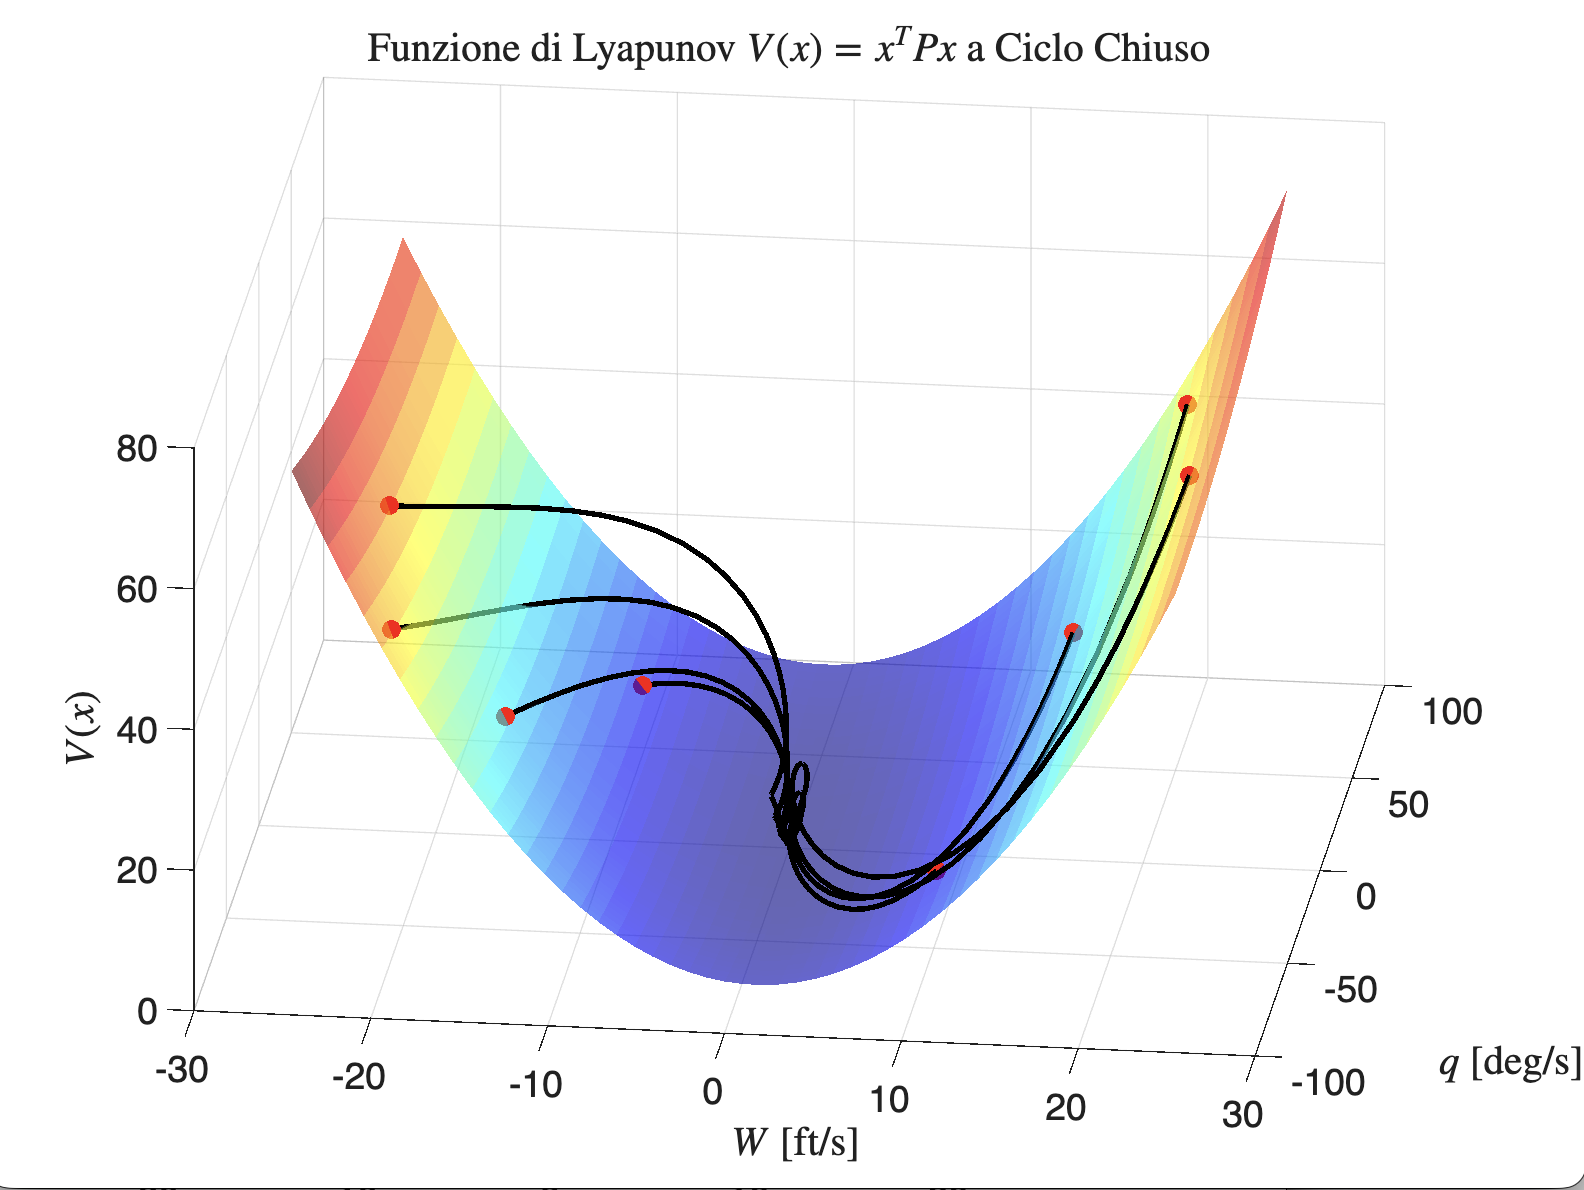
\includegraphics[width=0.7\linewidth]{Foto/photo/ljapunovDimostrativa}
	\caption{}
	\label{fig:ljapunov}
\end{figure}


\subsection{Applicazione della Regola di Bryson}
Per  avere un controllo realistico per la fisica dell' aereo il controllore adotta la \textbf{Regola di Bryson}\cite{Astrom2008}. Questo approccio prevede di costruire le matrici $Q$ ed $R$ come matrici diagonali, i cui elementi non nulli sono inversamente proporzionali al quadrato della massima variazione tollerabile per la rispettiva variabile:
\begin{equation}
	Q_{ii} = \frac{1}{(x_{i,\text{max}})^2}, \quad R_{jj} = \frac{1}{(u_{j,\text{max}})^2}
\end{equation}
quindi quando una variabile di stato o di controllo raggiunge il proprio limite fisico massimo il suo contributo all'indice di costo $J$ è normalizzato esattamente a 1. Sulla base delle caratteristiche fisiche dell'F-16, venogno utilizzatii i seguenti limiti per le variabili di stato del controllo longitudinale:
\begin{itemize}
	\item Angolo di beccheggio ($\theta$): $\theta_{\text{max}} = 15^\circ \approx 0.2618 \text{ rad}$
	\item Rateo di beccheggio ($q$): $q_{\text{max}} = 30^\circ/\text{s} \approx 0.5236 \text{ rad/s}$
	\item Velocità asse X ($U$): $U_{\text{max}} = 30 \text{ ft/s}$
	\item Velocità asse Z ($W$): $W_{\text{max}} = 20 \text{ ft/s}$
\end{itemize}

Dunque, la matrice $Q$ che si ottiene risulta:
\begin{equation}
	Q = \text{diag}\left( \frac{1}{(0.2618)^2}, \frac{1}{(0.5236)^2}, \frac{1}{(30)^2}, \frac{1}{(20)^2} \right)
\end{equation}

In modo analogo il vettore di controllo $u = [\delta_{\text{th}}, \delta_e, \delta_{\text{lef}}]^T$, i limiti fisici degli attuatori impongono:
\begin{itemize}
	\item Variazione di Spinta ($\delta_{\text{th}}$): $\text{Thrust}_{\text{max}} = 5000 \text{ lbs}$
	\item Equilibratore ($\delta_e$): $\text{Elev}_{\text{max}} = 25^\circ \approx 0.4363 \text{ rad}$
	\item Flap bordo d'attacco ($\delta_{\text{lef}}$): $\text{LEF}_{\text{max}} = 25^\circ \approx 0.4363 \text{ rad}$
\end{itemize}

La matrice di peso sulle azioni di controllo $R$ diviene quindi:
\begin{equation}
	R = \text{diag}\left( \frac{1}{(5000)^2}, \frac{1}{(0.4363)^2}, \frac{1}{(0.4363)^2} \right)
\end{equation}

\subsection{Conclusioni sulla sintesi LQR}
L'adozione della Regola di Bryson ha permesso di ricondurre il problema matematico dell'ottimizzazione quadratica a un significato puramente fisico e più realistico. Il controllore LQR così sintetizzato distribuisce l'energia di controllo in maniera ottimale, reagendo in modo bilanciato sia alle perturbazioni aerodinamiche lente che ai moti transitori veloci di beccheggio. La conferma visiva nel ritratto di fase della funzione di Lyapunov $V(x) = x^T P x$. Con la  normalizzazione, la mappa di energia nello spazio degli stati assume la conformazione teorica di un paraboloide, confermando che l'algoritmo sta valutando e penalizzando l'energia del sistema tenendo contro della fisica dell'aereo e delle diverse unità di misura delle variabili di stato.
% --- PRIMO CASO ---
\clearpage
\subsection{Prestazioni Aggressive Con Matrice Q dominante}
Sbilanciando la taratura a favore della matrice $Q$ (\textit{State Penalty}), la priorità del controllore è azzerare l'errore degli stati nel minor tempo matematicamente possibile. La richiesta di un rientro immediato genera comandi estremamente repentini. In questo scenario emerge la criticità dell'LQR: richiedendo un'azione di controllo troppo aggressiva per rimettere l'aereo in asse, i comandi teorici generati dal guadagno $K$ rischiano di superare ampiamente le reali capacità fisiche delle superfici aerodinamiche, mandando gli attuatori in saturazione e degradando la stabilità reale del velivolo. Il comportamento dinamico è illustrato nella Figura \ref{fig:lqr_q_dominante}.

\begin{figure}[!h]
	\centering
	\begin{subfigure}[b]{0.48\textwidth}
		\centering
		\includegraphics[width=\textwidth]{Foto/photo/LQRQdominant_Stati}
		\caption{Dinamica degli stati a ciclo chiuso.}
		\label{fig:lqrqdominantstati}
	\end{subfigure}
	\hfill
	\begin{subfigure}[b]{0.48\textwidth}
		\centering
		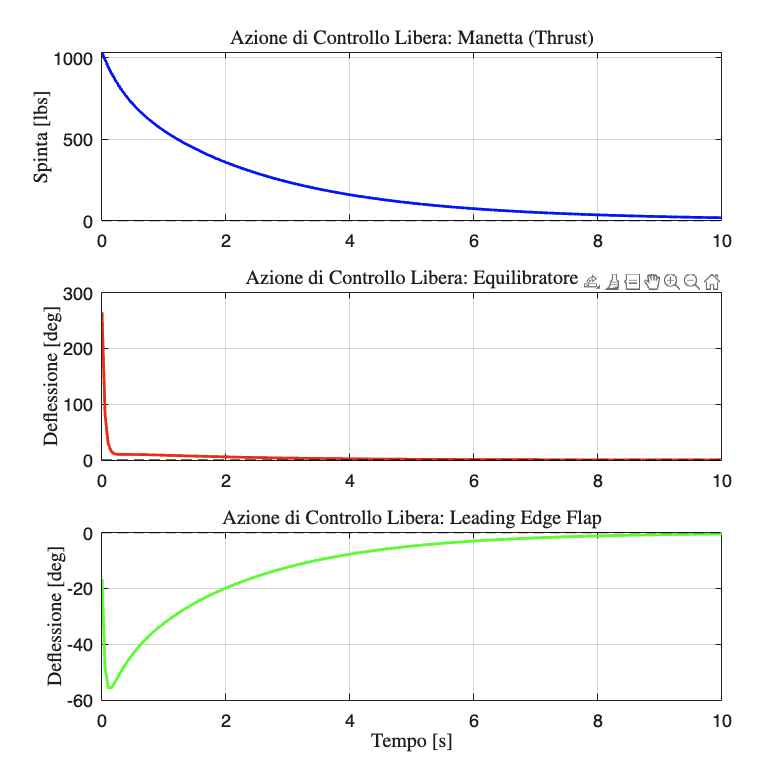
\includegraphics[width=\textwidth]{Foto/photo/LQRQdominantAttutatori.png}
		\caption{Sforzo di controllo richiesto agli attuatori.}
		\label{fig:lqrqdominantattuatori}
	\end{subfigure}
	\caption{Risposta del sistema con $Q \gg R$. (a) Il rientro è immediato e aggressivo,(b) ma genera picchi di comando che possono causare la saturazione degli attuatori.}
	\label{fig:lqr_q_dominante}
\end{figure}

\begin{figure}[!h]
	\centering
	\begin{subfigure}[b]{0.48\textwidth}
		\centering
		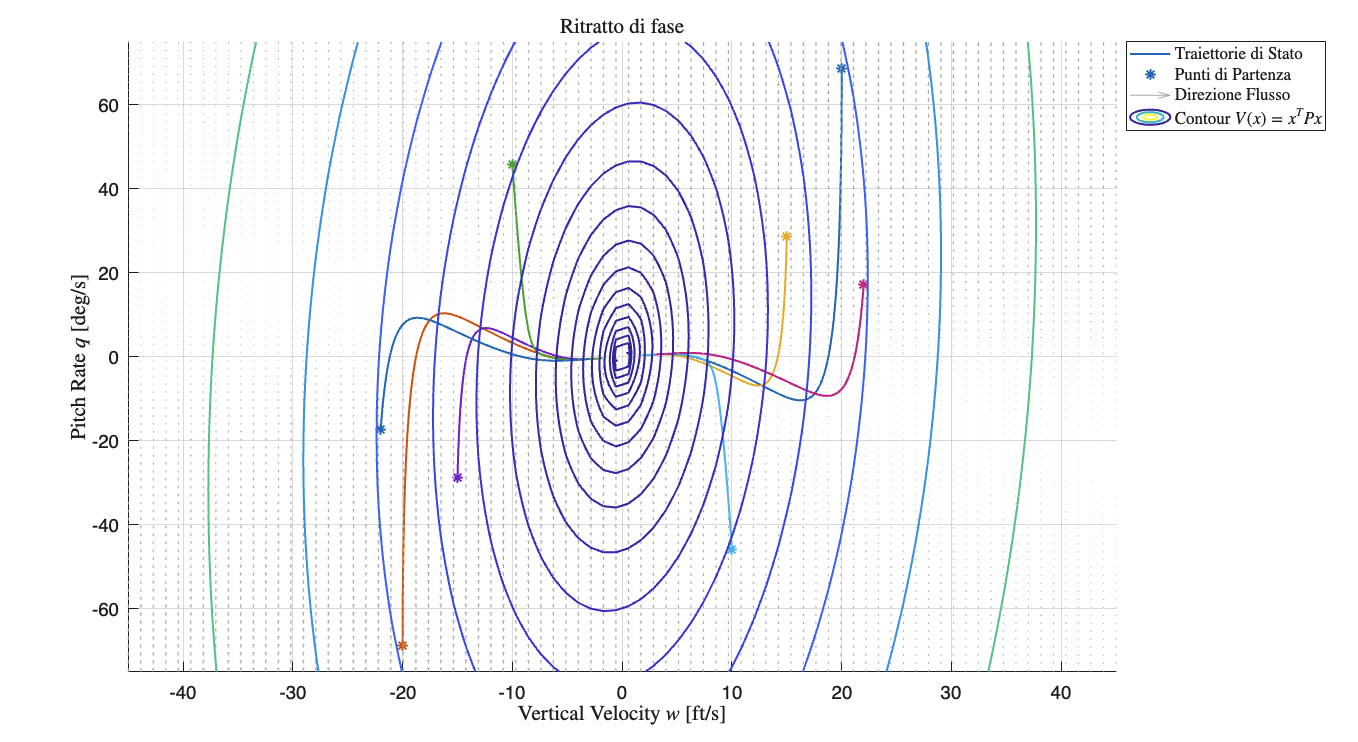
\includegraphics[width=\textwidth]{Foto/mpc/QaggressiveFase.png}
		\caption{Ritratto di fase del sistema.}
		\label{fig:lqrqdominant_fase}
	\end{subfigure}
	\hfill
	\begin{subfigure}[b]{0.48\textwidth}
		\centering
		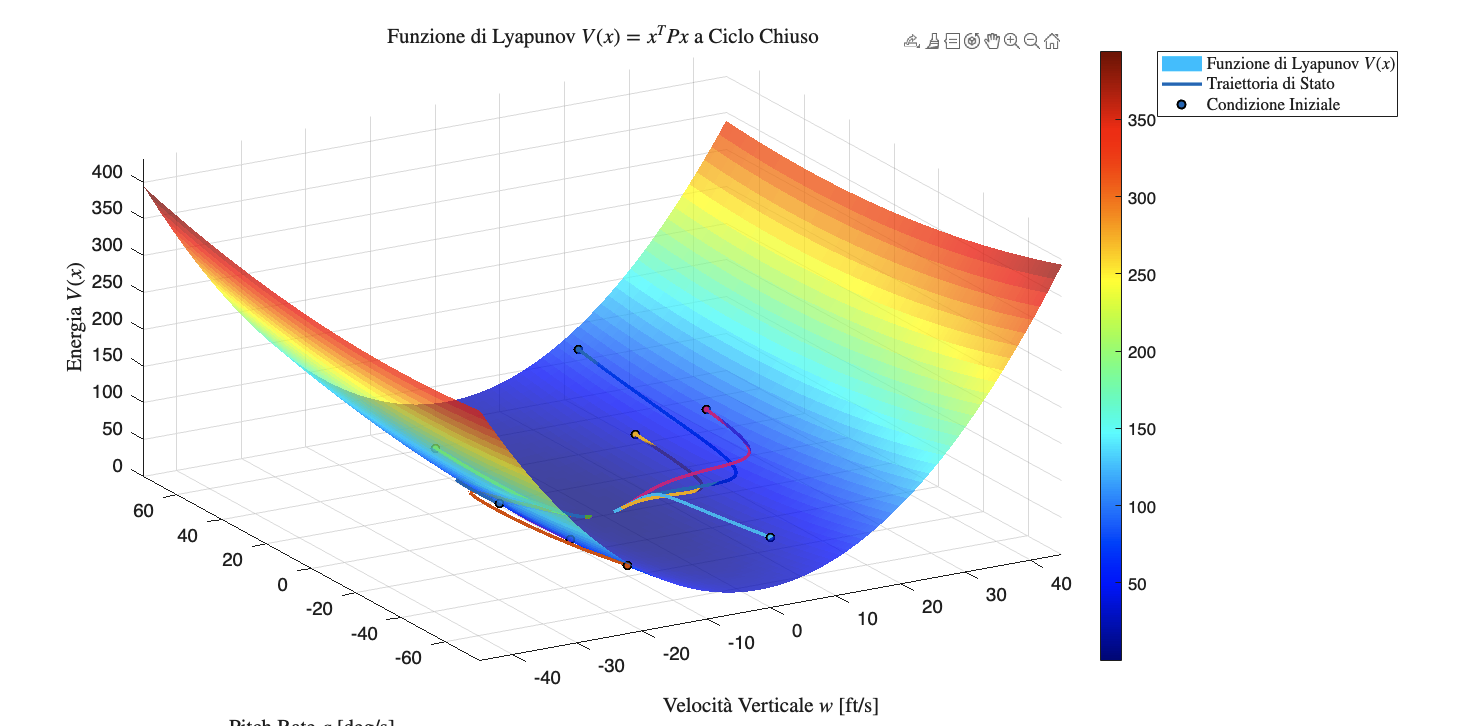
\includegraphics[width=\textwidth]{Foto/mpc/Qljapunov.png}
		\caption{Superficie 3D della funzione di Lyapunov.}
		\label{fig:lqrqdominant_lyapunov}
	\end{subfigure}
	\caption{Analisi geometrica con $Q \gg R$. La ripidezza della funzione di Lyapunov (b) forza le traiettorie di fase (a) a una convergenza dalle condizioni inziali verso l'equilibrio.}
	\label{fig:lqr_q_dominante_fase_lyap}
\end{figure}

Valutando l'analisi dinamica si nota che il comportamento del sistema può essere valutato  attraverso il ritratto di fase e la forma quadratica della funzione ottima di Lyapunov utilizzata, definita come $V(x) = x^T P x$ (dove $P$ è la soluzione dell'Equazione Algebrica di Riccati), quindi i grafici che vengono plottati cambieranno in base a come vengono penalizzate le matrici Q ed R. In questo scenario aggressivo, la superficie 3D di Lyapunov si presenta particolarmente ripida e scavata, riflettendo l'elevato costo associato alla deviazione degli stati dall'equilibrio. Il ritratto di fase evidenzia traiettorie che precipitano verso l'origine con pendenze elevate: la convergenza è estremamente rapida, ma la geometria delle curve conferma l'assenza di smorzamento graduale, sintomo della forte richiesta energetica che il sistema richiede.
Valutando l'analisi dinamica si nota che el comportamento del sistema può essere valutato  attraverso el ritratto di fase e la forma quadratica della funzione ottima di Lyapunov utilizzata, definita come $V(x) = x^T P x$ (dove $P$ è la soluzione dell'Equazione Algebrica di Riccati), quindi i grafici che vengono plottati cambieranno in base a come vengono penalizzate le matrici Q ed R. In questo scenario aggressivo, la superficie 3D di Lyapunov si presenta particolarmente ripida e scavata, riflettendo l'elevato costo associato alla deviazione degli stati dall'equilibrio. El ritratto di fase evidenzia traiettorie che precipitano verso l'origine con pendenze elevate: la convergenza è estremamente rapida, ma la geometria delle curve conferma l'assenza di smorzamento graduale, sintomo della forte richiesta energetica che el sistema richiede.

\clearpage
% --- SECONDO CASO ---
\subsection{Compromesso Ottimo Con Matrici Q ed R bilanciate}
Per ottenere un comportamento realistico e applicabile in volo, è necessario individuare un bilanciamento tra le due matrici ($Q \approx R$, al netto delle dovute normalizzazioni di scala). In questo scenario di compromesso, l'LQR fornisce la sua prestazione ottimale: garantisce un rientro sufficientemente rapido dell'assetto e lo smorzamento delle oscillazioni (tipiche del modo Phugoide e Corto Periodo), mantenendo contemporaneamente le richieste di deflessione dell'equilibratore entro limiti operativi sicuri. Questo set di guadagni, analizzato nella Figura \ref{fig:lqr_bilanciato}, rappresenta la taratura nominale scelta per el controllore a ciclo chiuso.

	\begin{figure}[H]
		\centering
		\begin{subfigure}[b]{0.48\textwidth}
			\centering
			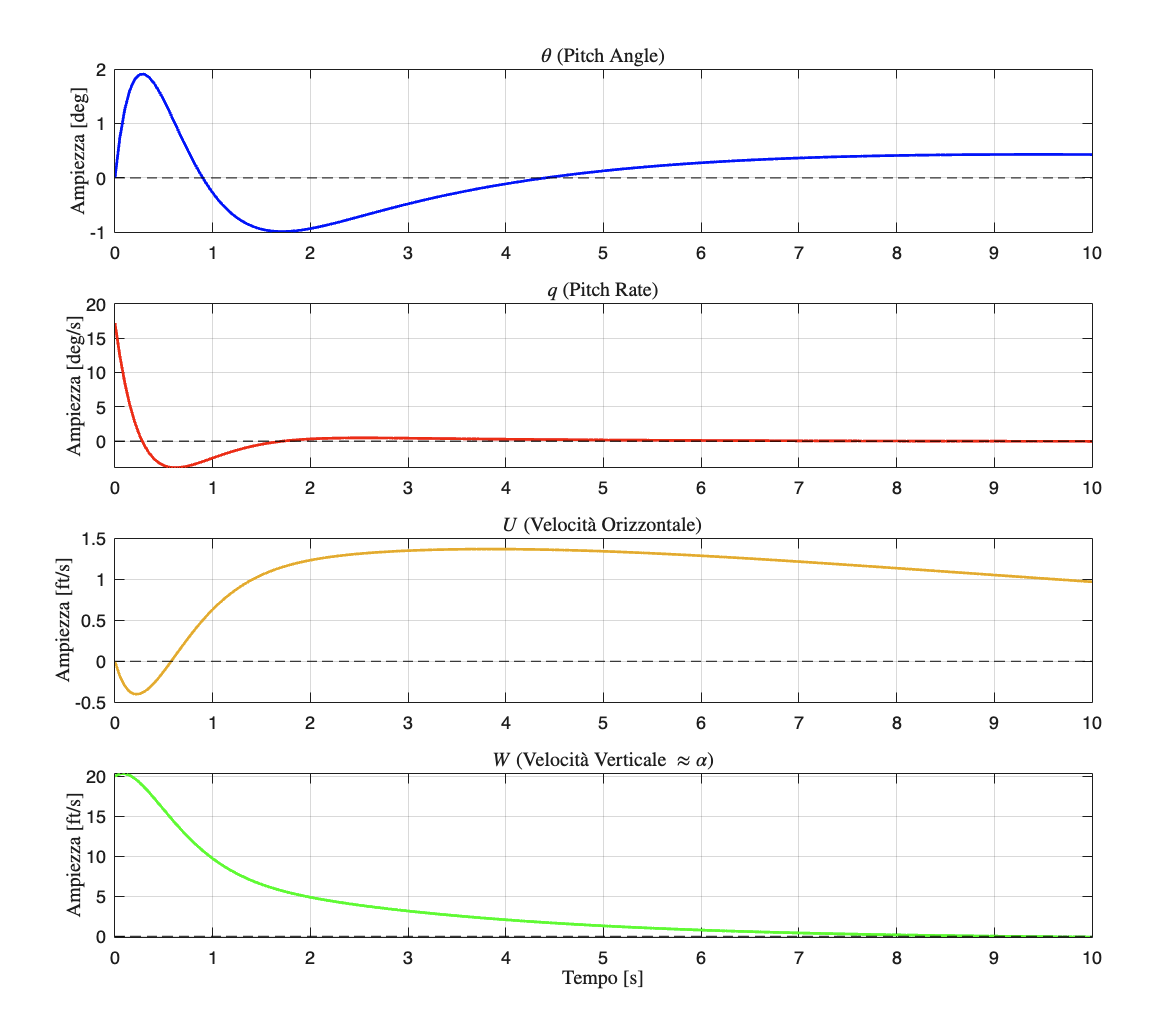
\includegraphics[width=\textwidth]{Foto/photo/LQREqual_Stati}
			\caption{Dinamica degli stati a ciclo chiuso.}
			\label{fig:lqrEqual_Stati}
		\end{subfigure}
		\hfill
		\begin{subfigure}[b]{0.48\textwidth}
			\centering
			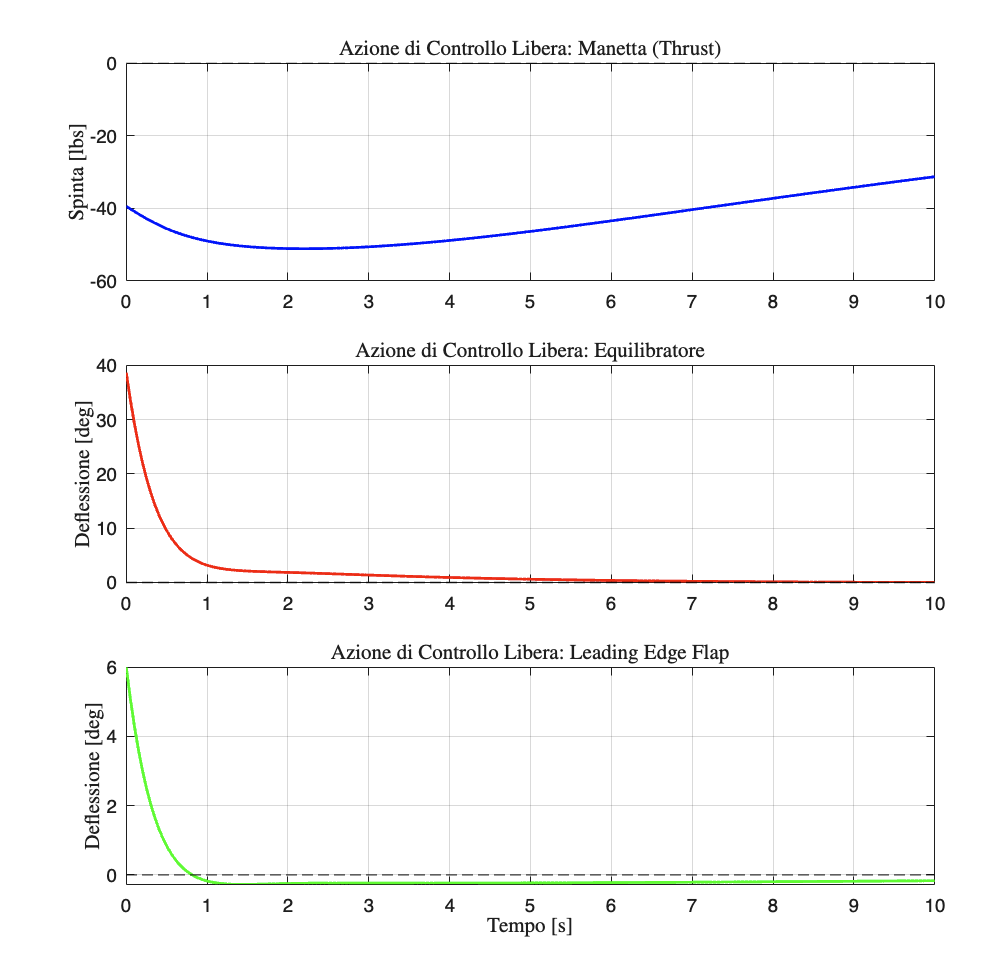
\includegraphics[width=\textwidth]{Foto/photo/LQREqual_Att.png}
			\caption{Sforzo di controllo richiesto agli attuatori.}
			\label{fig:lqrEqual_Attuatori}
		\end{subfigure}
		\caption{Risposta del sistema con $Q \approx R$. El controllore offre un ottimo compromesso tra rapidità di reiezione del disturbo (a) e contenimento dello sforzo di controllo (b).}
		\label{fig:lqr_bilanciato}
	\end{figure}

L'efficacia di questo compromesso si riflette in modo evidente nella topologia dello spazio degli stati. Osservando la funzione di Lyapunov per el caso bilanciato, si nota una conformazione della superficie 3D più armoniosa e ben proporzionata. La discesa delle traiettorie di stato lungo la "conca" definita da $V(x)$ avviene in modo fluido e diretto verso el punto di equilibrio. El ritratto di fase conferma l'ottimo smorzamento introdotto dal controllore: le traiettorie spiraleggiano o convergono stabilmente verso l'origine senza le deviazioni brusche del caso precedente, garantendo stabilità senza stressare l'aerodinamica del velivolo.

\begin{figure}[H]
	\centering
	\begin{subfigure}[b]{0.48\textwidth}
		\centering
		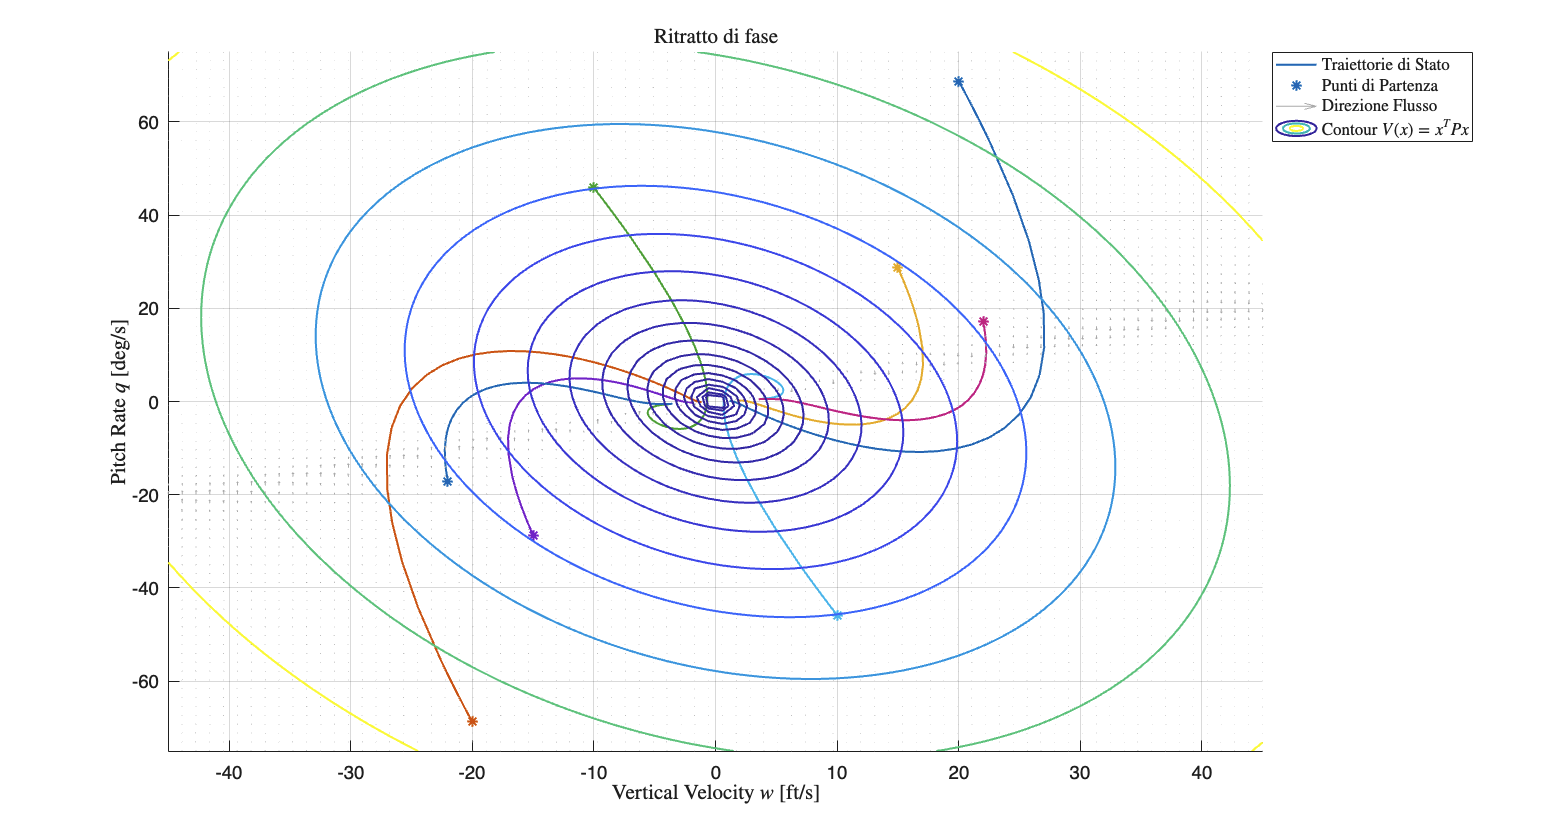
\includegraphics[width=\textwidth]{Foto/mpc/EqualFase.png}
		\caption{Ritratto di fase del sistema.}
		\label{fig:lqrEqual_Fase}
	\end{subfigure}
	\hfill
	\begin{subfigure}[b]{0.48\textwidth}
		\centering
		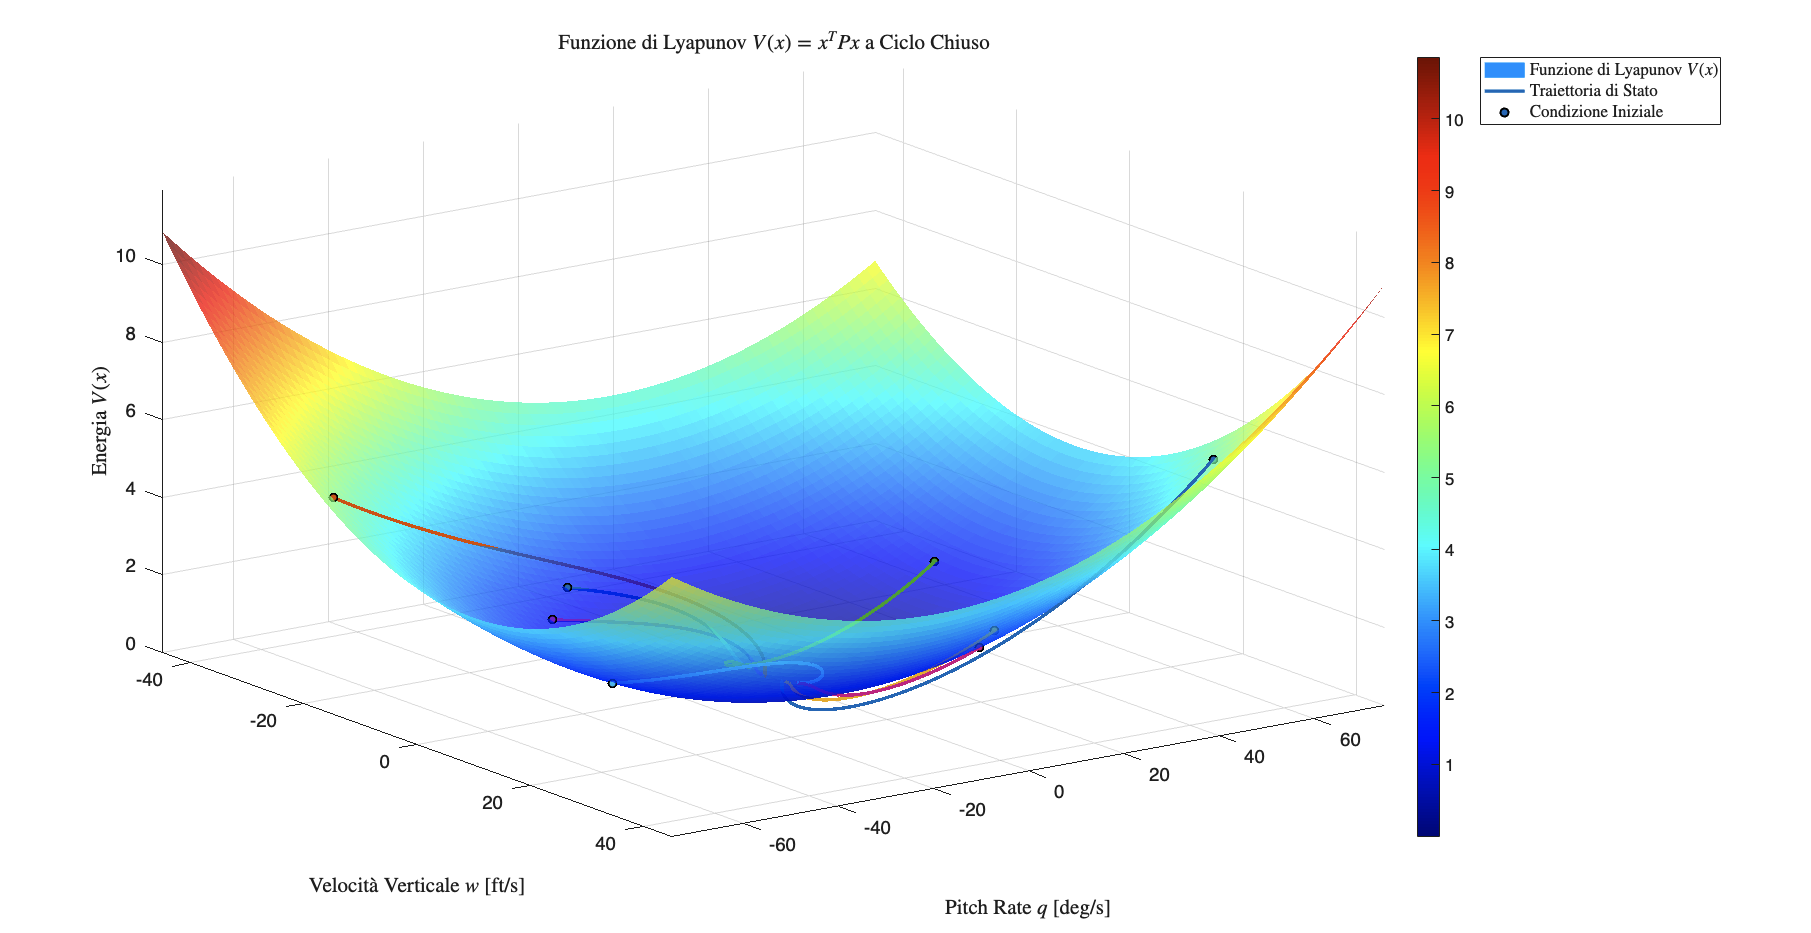
\includegraphics[width=\textwidth]{Foto/mpc/EquaLjapunov.png}
		\caption{Superficie 3D della funzione di Lyapunov.}
		\label{fig:lqrEqual_Lyapunov}
	\end{subfigure}
	\caption{Analisi geometrica con $Q \approx R$. La conformazione bilanciata della superficie di Lyapunov (b) garantisce traiettorie di fase (a) fluide e ben smorzate verso l'origine.}
	\label{fig:lqr_bilanciato_fase_lyap}
\end{figure}

% --- TERZO CASO ---
\subsection{Risparmio Energetico Con Matrice R dominante}
All'estremo opposto, impostando valori elevati sulla diagonale della matrice $R$ (\textit{Control Penalty}), l'algoritmo di ottimizzazione penalizza fortemente l'utilizzo degli attuatori rispetto all'errore di stato. La priorità del solutore è il risparmio di energia di manovra: l'azione di controllo dell'equilibratore risulta dolce e priva di picchi. Di conseguenza, il controllore accetta un transitorio molto più lungo per riportare l'aereo nel punto di equilibrio, lasciando decadere le perturbazioni gradualmente ed evitando qualsiasi rischio di saturazione, a discapito della prontezza di risposta. I risultati sono riportati nella Figura \ref{fig:lqr_r_dominante}. Coerentemente con la penalizzazione dello sforzo di controllo, la topologia del sistema subisce una variazione significativa. La predominanza della matrice $R$ si traduce in una funzione ottima di Lyapunov molto "piatta" e con pendenze dolci. Poiché il costo associato all'errore di stato è marginale, il solutore permette alle traiettorie nel ritratto di fase di compiere ampie escursioni prima di chiudersi sull'origine. La discesa lungo la superficie 3D avviene con estrema lentezza: il sistema scivola dolcemente verso il punto operativo, privilegiando la totale minimizzazione dello sforzo di deflessione rispetto alla prontezza aerodinamica.

\begin{figure}[!h]
	\centering
	\begin{subfigure}[b]{0.48\textwidth}
		\centering
		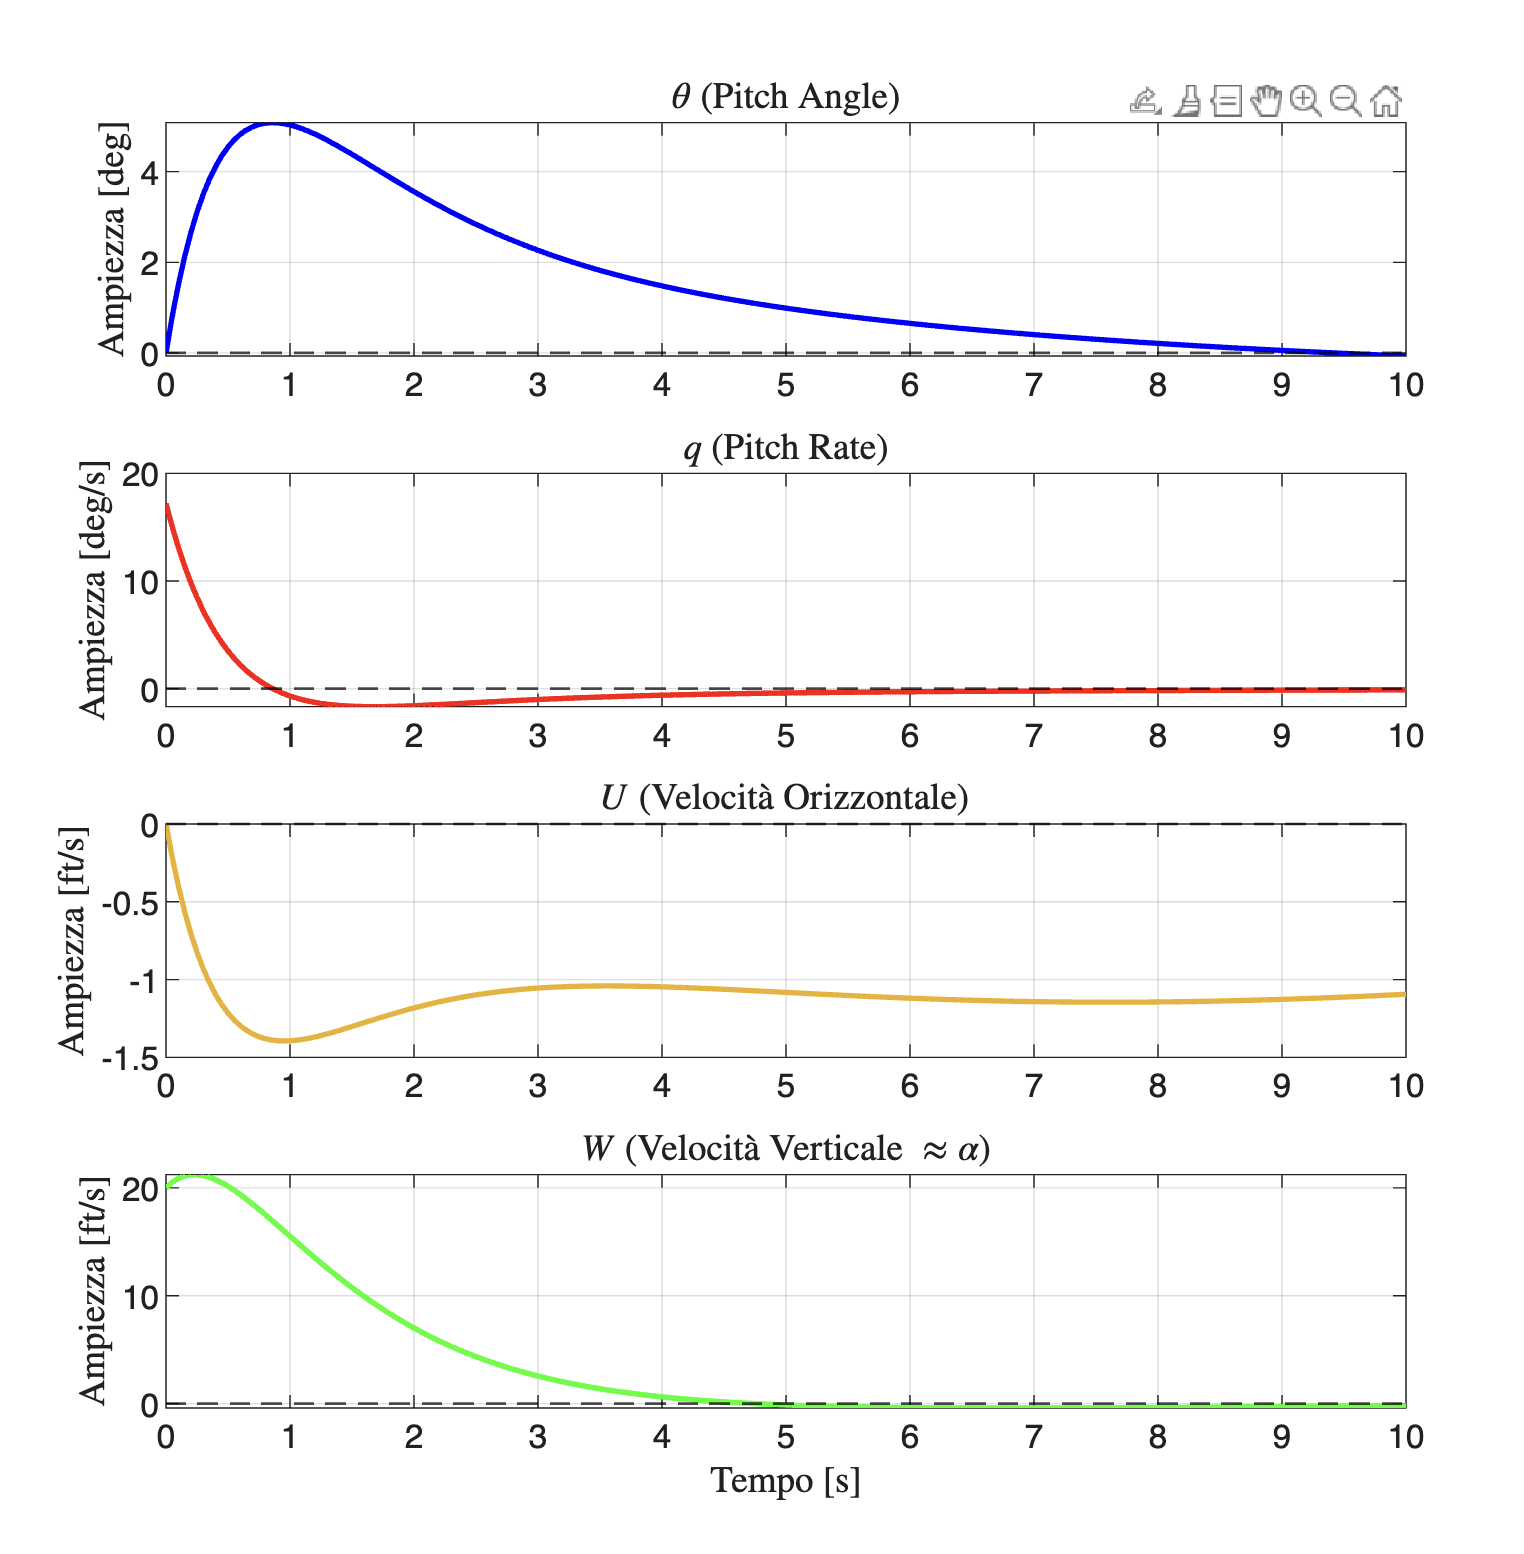
\includegraphics[width=\textwidth]{Foto/photo/LQRRdominant_Stati}
		\caption{Dinamica degli stati a ciclo chiuso.}
		\label{fig:lqrRdominant_Stati}
	\end{subfigure}
	\hfill
	\begin{subfigure}[b]{0.48\textwidth}
		\centering
		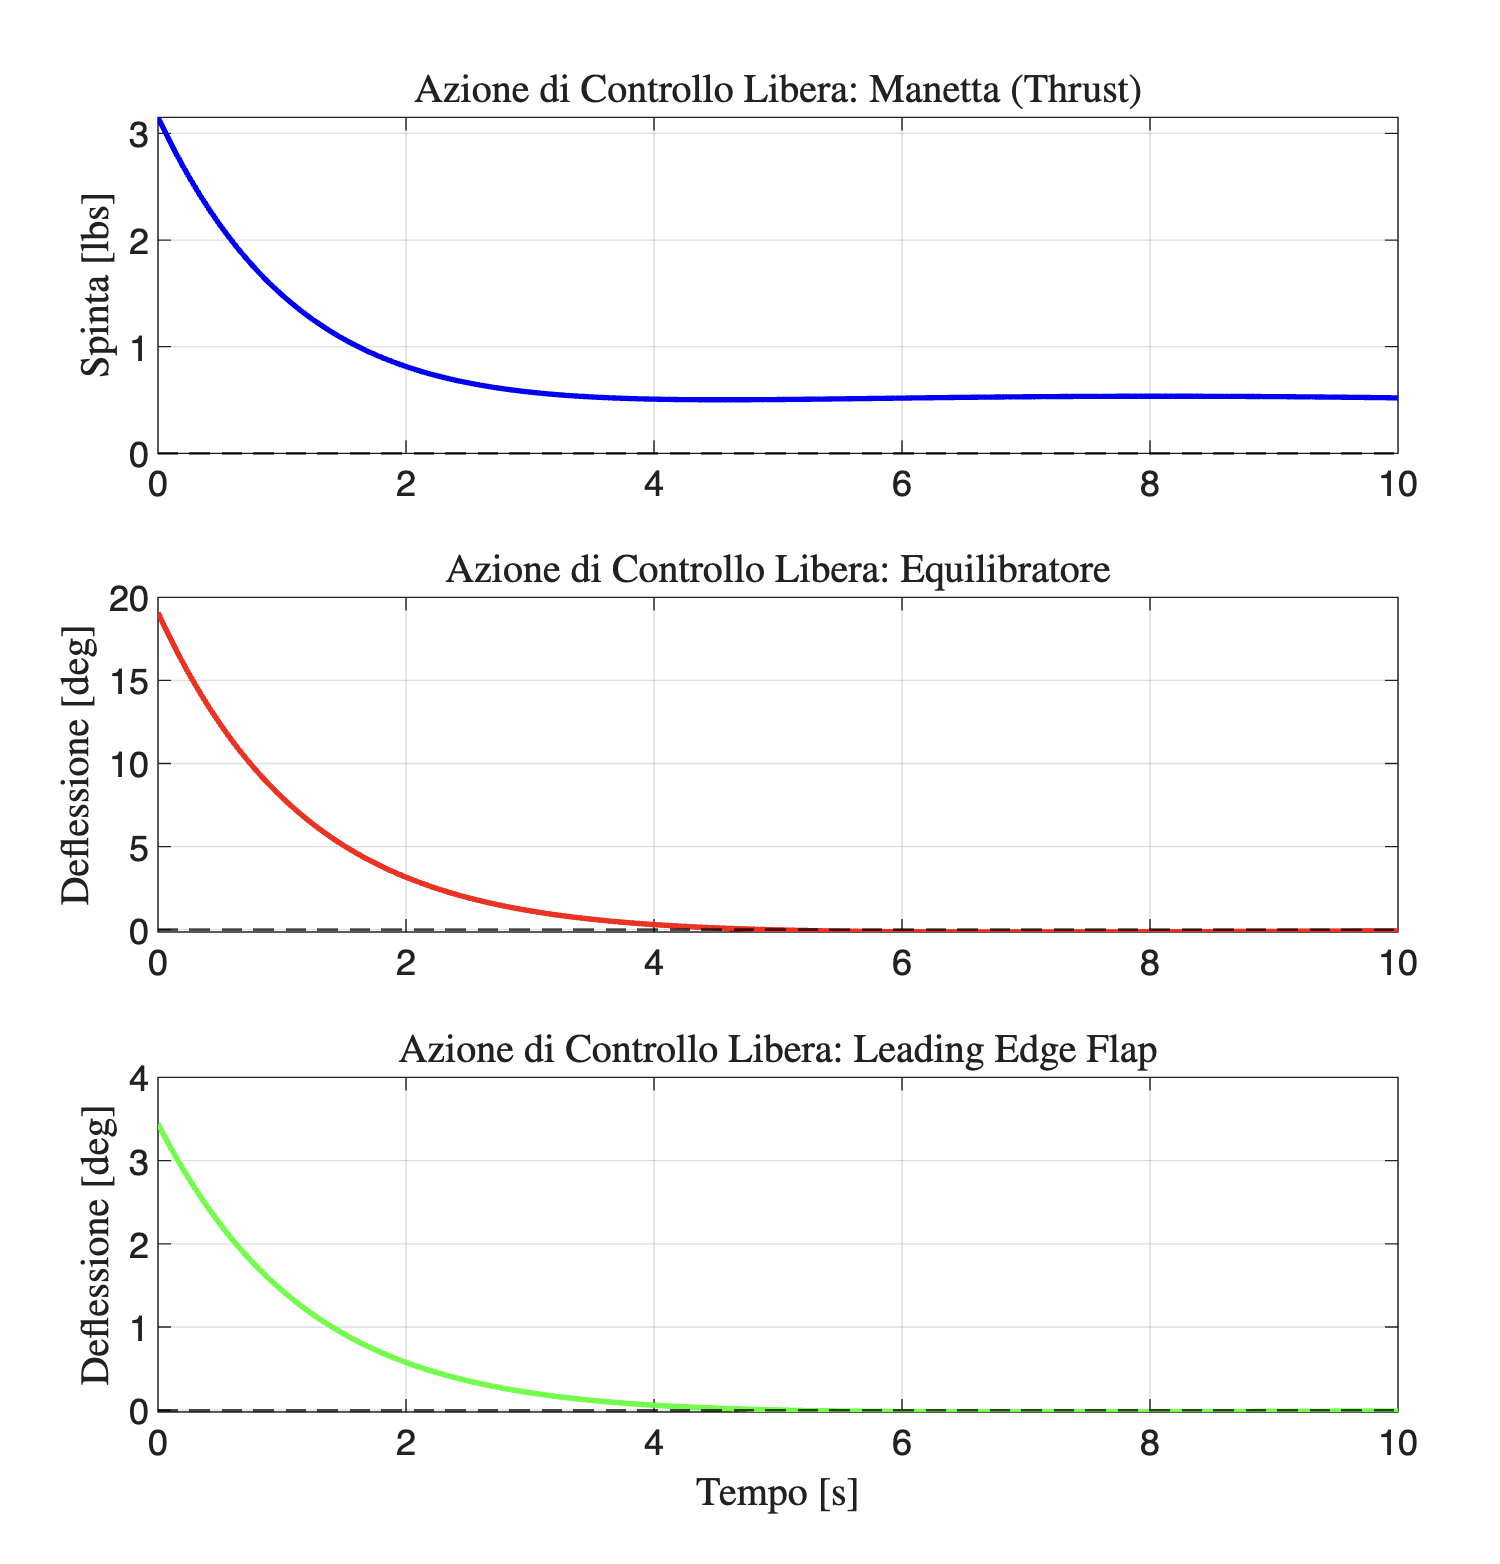
\includegraphics[width=\textwidth]{Foto/photo/LQRRdominant_Attutatori.png}
		\caption{Sforzo di controllo richiesto agli attuatori.}
		\label{fig:lqrRdominant_Attuatori}
	\end{subfigure}
	\caption{Risposta del sistema con $R \gg Q$. L'azione di controllo è moderata ed energeticamente efficiente (b), ma il rientro al punto operativo risulta molto più lento (a).}
	\label{fig:lqr_r_dominante}
\end{figure}



\begin{figure}[!h]
	\centering
	\begin{subfigure}[b]{0.48\textwidth}
		\centering
		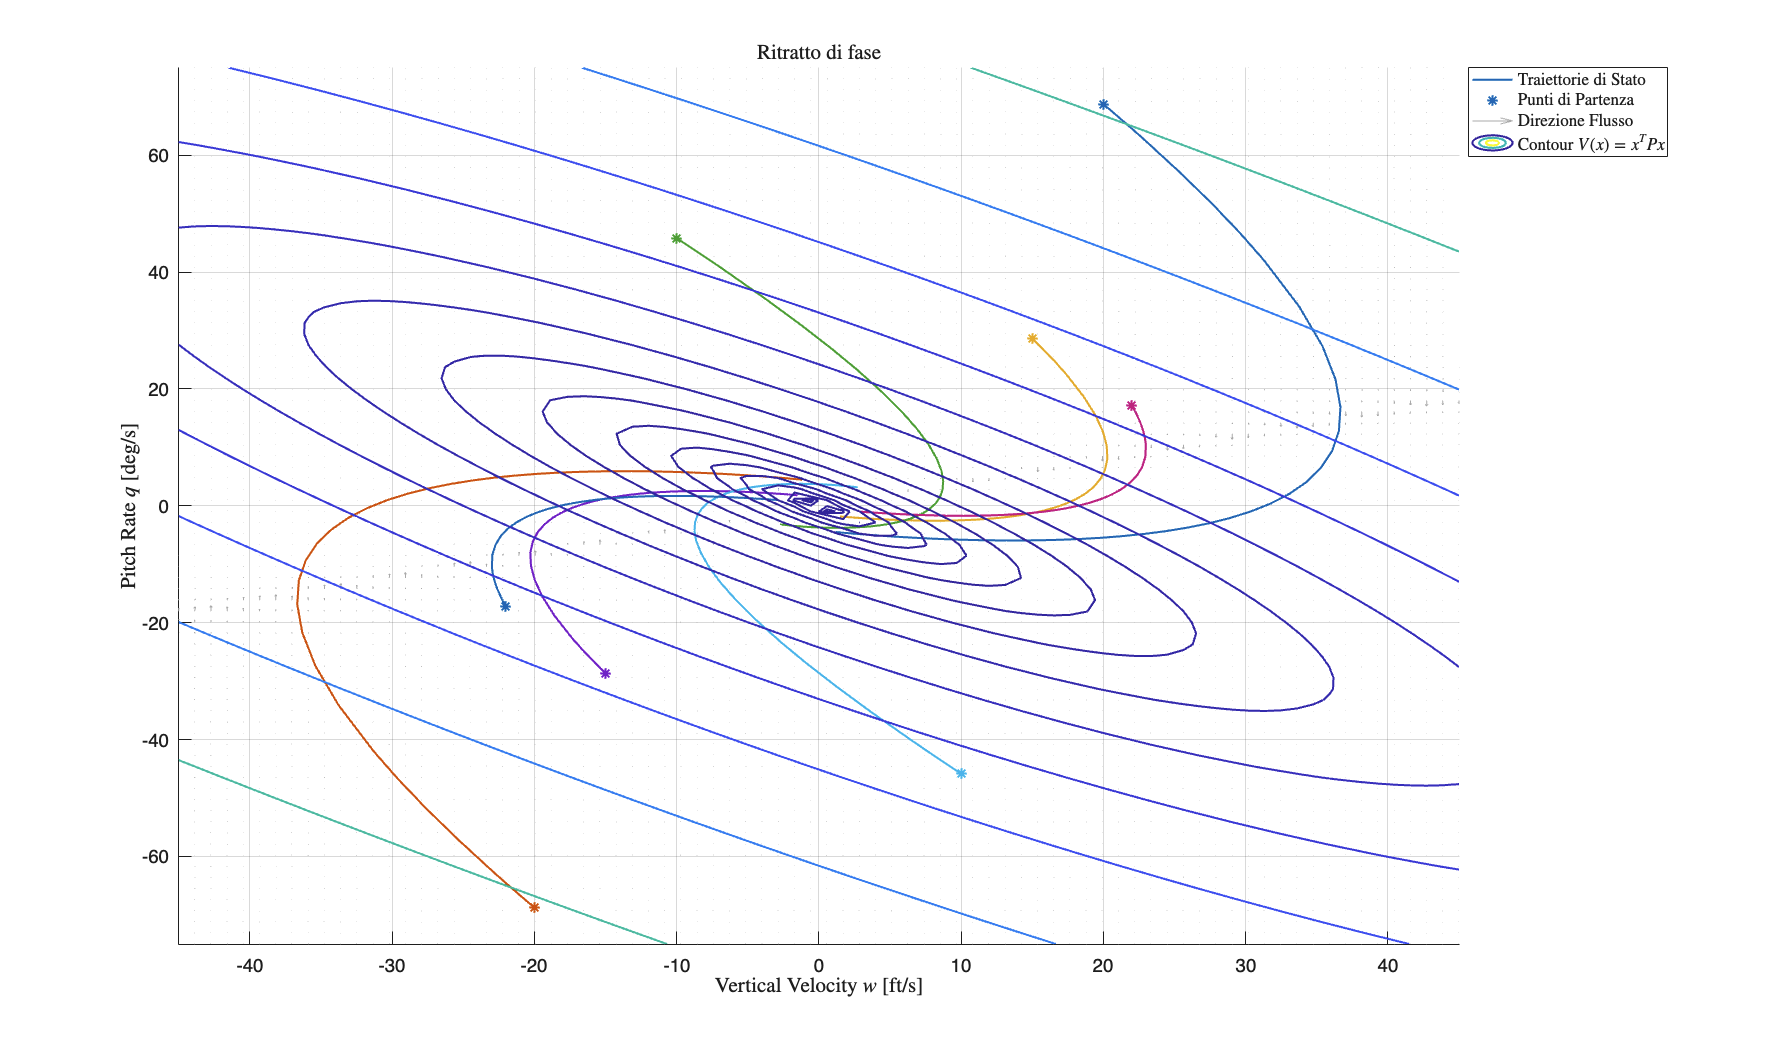
\includegraphics[width=\textwidth]{Foto/mpc/Rfase.png}
		\caption{Ritratto di fase del sistema.}
		\label{fig:lqrRdominant_Fase}
	\end{subfigure}
	\hfill
	\begin{subfigure}[b]{0.48\textwidth}
		\centering
		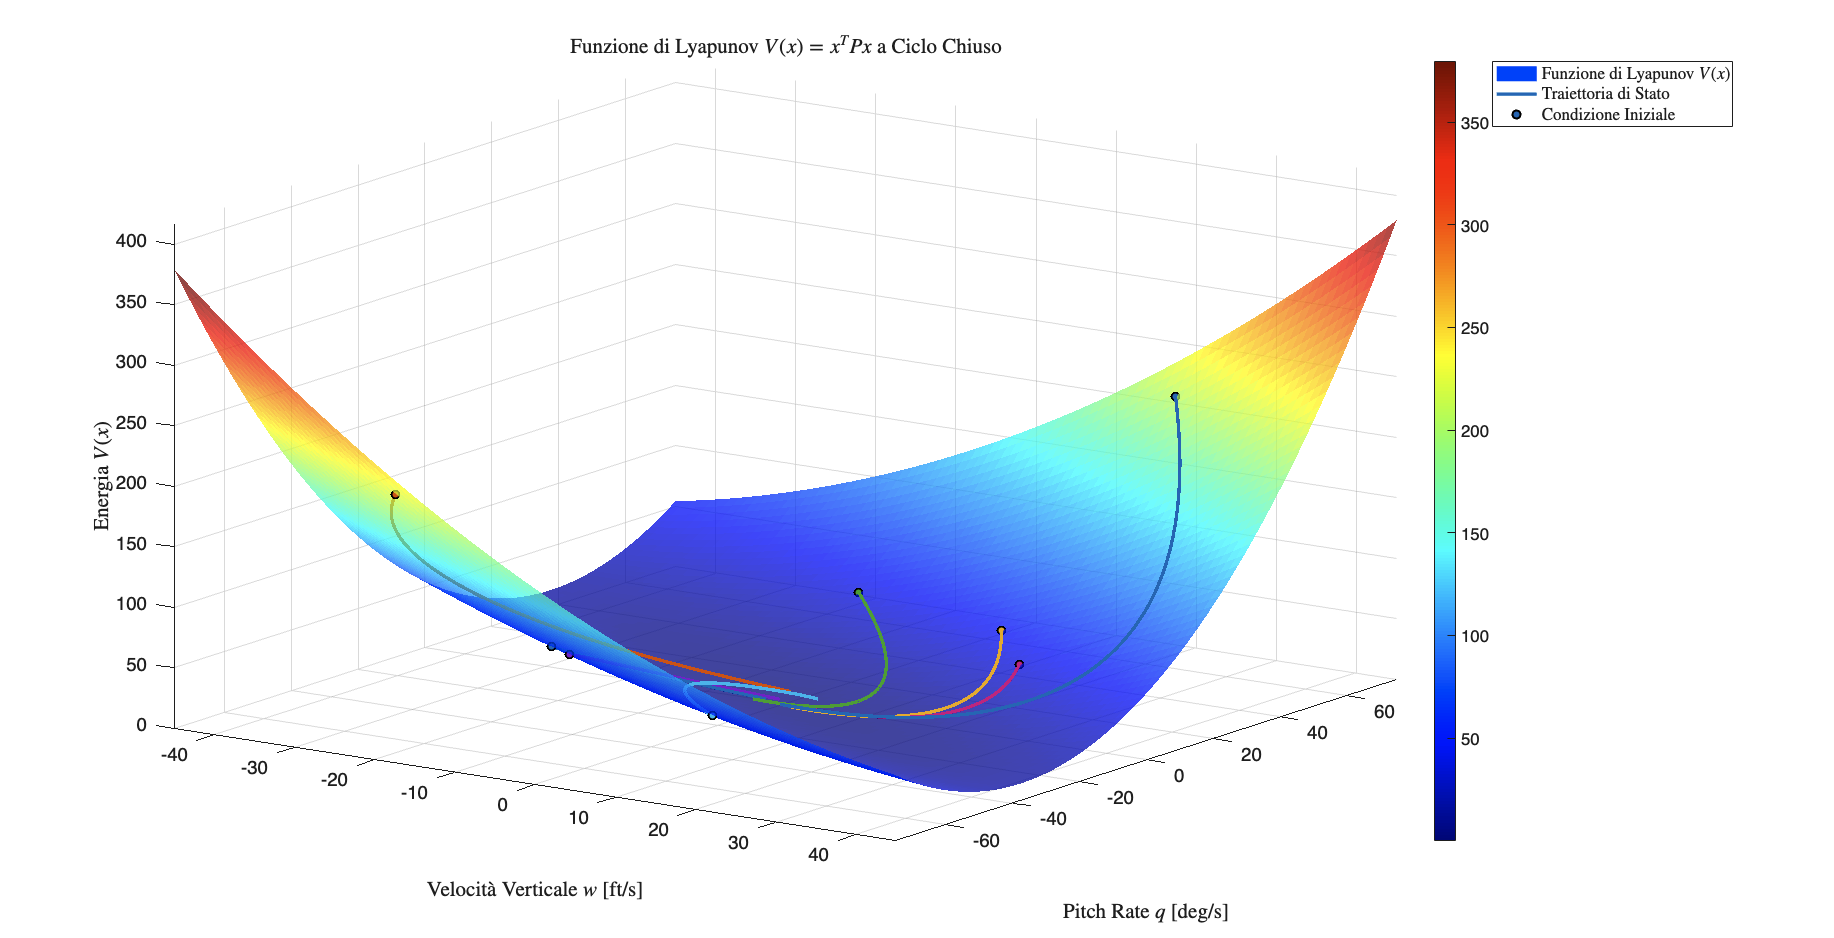
\includegraphics[width=\textwidth]{Foto/mpc/Rljapunov.png}
		\caption{Superficie 3D della funzione di Lyapunov.}
		\label{fig:lqrRdominant_Lyapunov}
	\end{subfigure}
	\caption{Analisi geometrica con $R \gg Q$. La superficie di Lyapunov risulta quasi piatta (b), permettendo alle traiettorie di fase (a) ampie escursioni e una convergenza molto lenta.}
	\label{fig:lqr_r_dominante_fase_lyap}
\end{figure}
\clearpage
